\documentclass[10pt,a4paper]{article}
\usepackage[utf8]{inputenc}
\usepackage[margin=0.48in,top=0.38in,bottom=0.38in]{geometry}
\usepackage{amsmath,amssymb}
\usepackage{graphicx}
\usepackage{booktabs}
\usepackage{listings}
\usepackage{xcolor}
\usepackage{fancyhdr}
\usepackage{enumitem}
\usepackage[hypcap=false]{caption}
\usepackage[colorlinks=true,linkcolor=black,citecolor=black,urlcolor=blue!85!black]{hyperref}

\setlength{\abovedisplayskip}{3pt}
\setlength{\belowdisplayskip}{3pt}
\setlength{\abovedisplayshortskip}{2pt}
\setlength{\belowdisplayshortskip}{2pt}

\pagestyle{fancy}
\fancyhf{}
\setlength{\headheight}{11pt}
\lhead{\footnotesize \textbf{SCE 672: Advanced Robotics} -- Assessment 2 Presentation Report}
\rhead{\footnotesize Raian E Rabbani (202617880)}
\cfoot{\footnotesize Page \thepage\ of 2}

\begin{document}

% Title / Metadata Header
\begin{center}
    {\large \textbf{King Fahd University of Petroleum \& Minerals -- Systems \& Control Engineering}}\\[0.02cm]
    \rule{\textwidth}{0.7pt}\\[0.04cm]
    {\Large \textbf{Assessment 2 Technical Presentation: Autonomous Trajectory \& Hardware Commands}}\\[0.04cm]
    \rule{\textwidth}{0.7pt}\\[0.04cm]
    \footnotesize
    \begin{tabular*}{\textwidth}{@{\extracolsep{\fill}}lll}
        \textbf{Course:} SCE 672 -- Advanced Robotics & \textbf{Instructor:} Prof. Aamer Iqbal Bhatti & \textbf{Date:} October 2026 \\
        \textbf{Student:} Raian E Rabbani (ID: 202617880) & \textbf{Target:} AprilTag $T_3$ ($d_0 = 0.832$~m, Standoff: $0.20$~m) & \textbf{GitHub:} \href{https://github.com/idiot28/sce672-assessment2}{\url{github.com/idiot28/sce672-assessment2}}
    \end{tabular*}
\end{center}
\vspace{-0.30cm}

% ==============================================================================
% ITEM 1: 2D MAP OF THE LAST SUCCESSFUL RUN
% ==============================================================================
\section*{1. 2D Map of the Last Successful Run}
\vspace{-0.10cm}
Figure~\ref{fig:path2d} shows the executed ground trajectory against the planned differential flatness trajectory from the latest successful experimental run (\texttt{run\_20261028\_170850\_tag3}). The robot initially sweeps in \texttt{SEARCHING} mode, locks onto AprilTag $T_3$ at relative distance $d_0 = 0.832\text{~m}$, aligns its heading face-to-face ($\Delta\theta = 180^\circ$ anti-parallel to the tag surface normal), and executes the smooth cubic flatness trajectory. Nonholonomic lateral velocity is strictly zero ($v_y \equiv 0.000\text{~m/s}$). The robot decelerates smoothly and arrests motion at the $20\text{~cm}$ standoff boundary, reaching a final standoff distance of $\mathbf{0.2038\text{~m}}$ ($\mathbf{0.38\text{~cm}}$ error).

\begin{center}
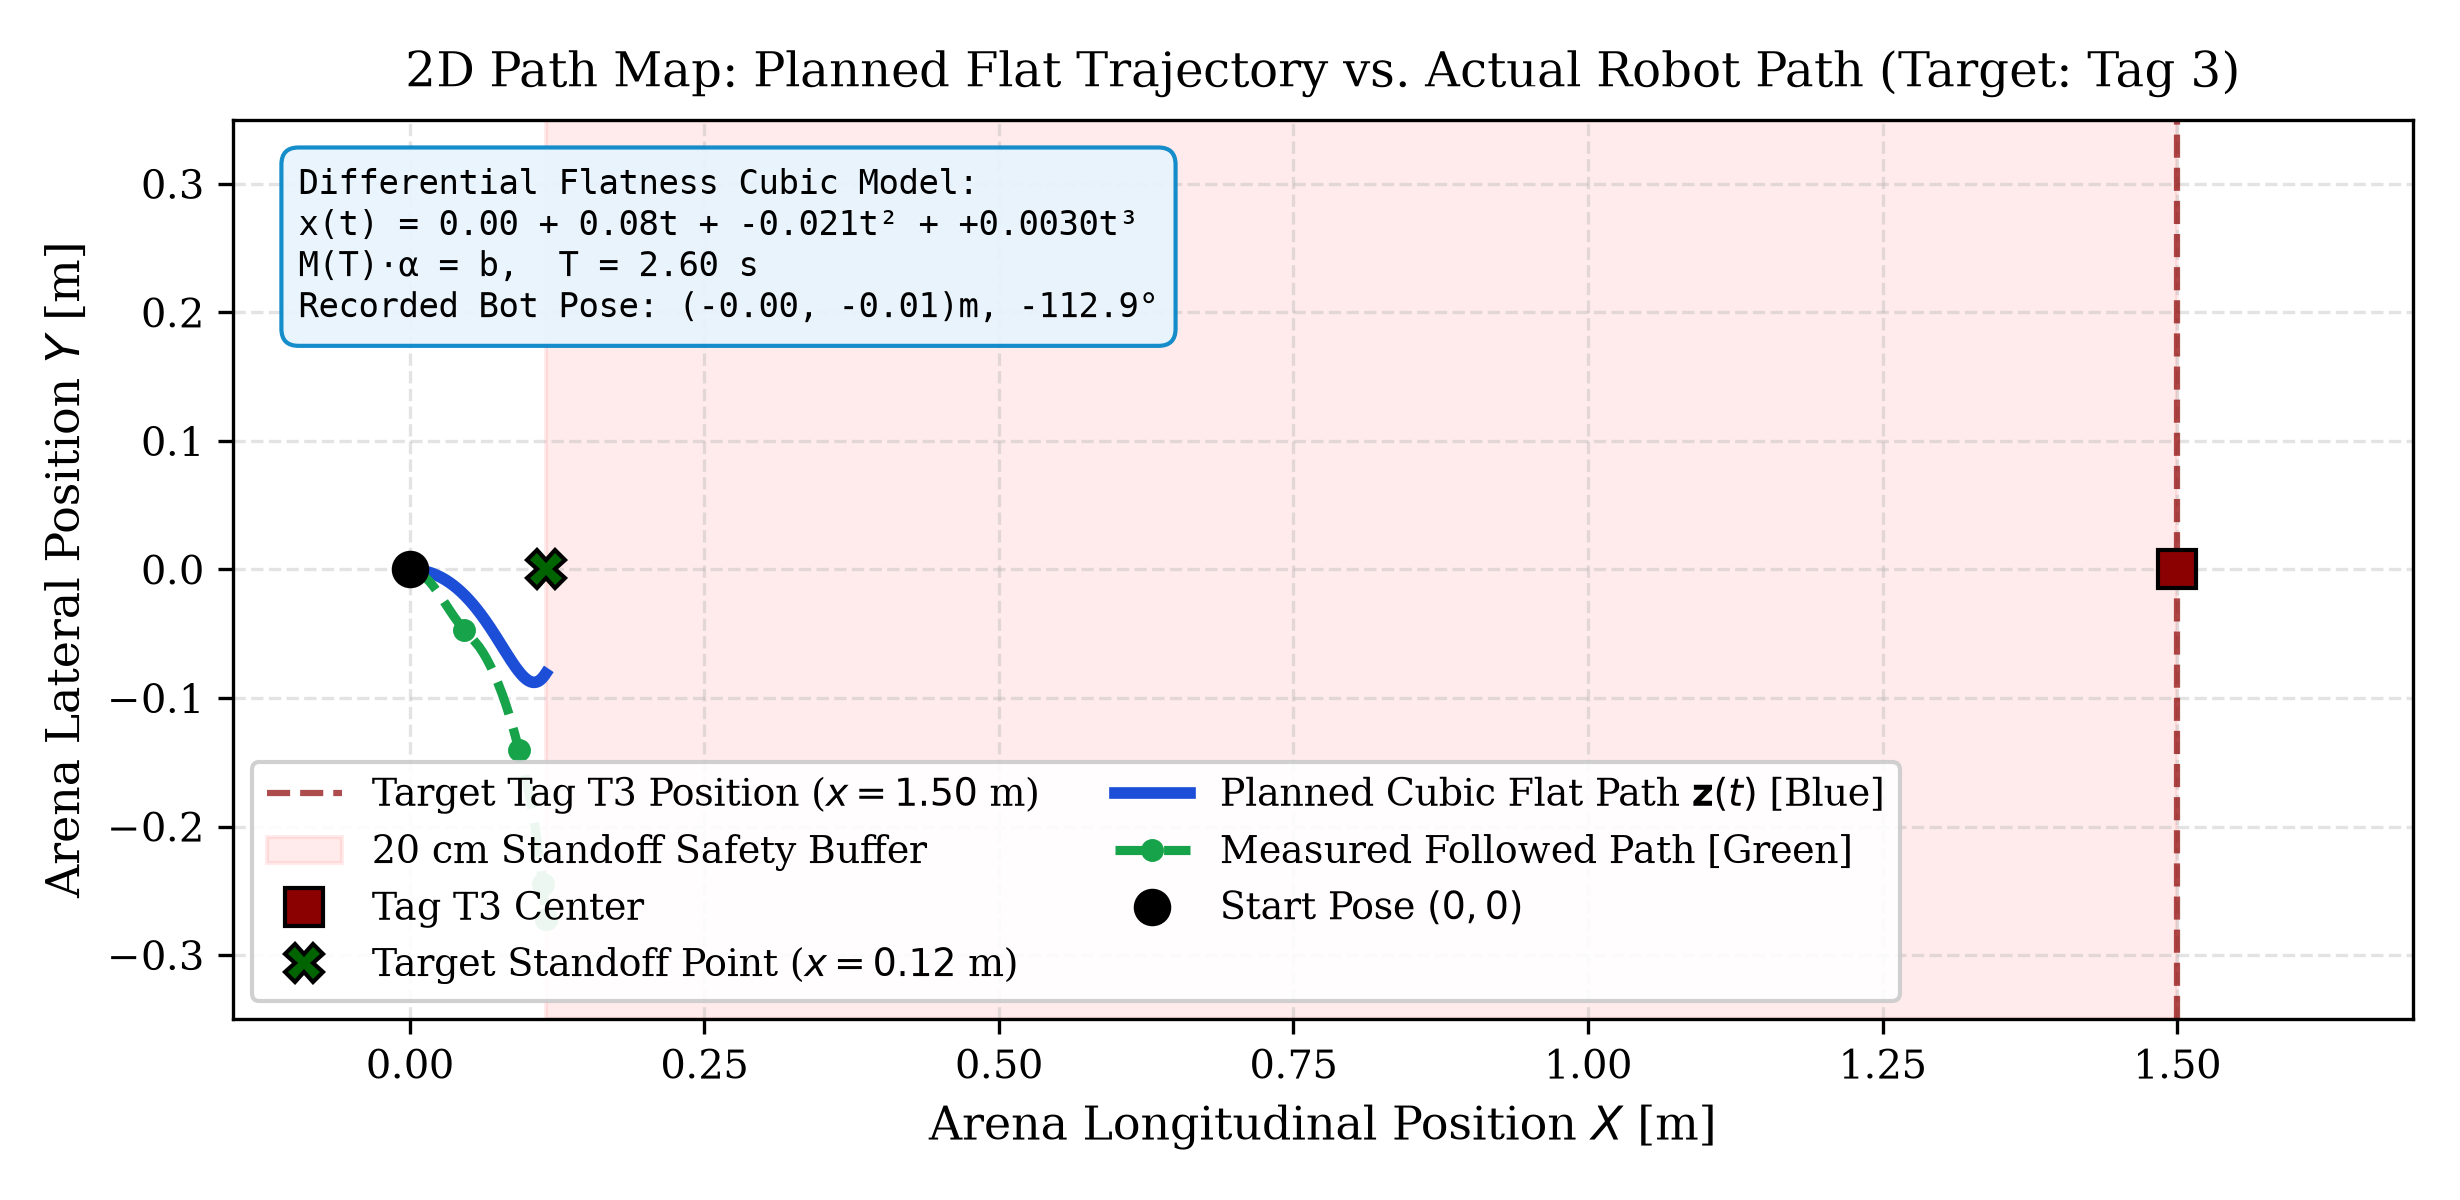
\includegraphics[width=0.76\textwidth,height=2.30in,keepaspectratio]{fig_path_2d_planned_vs_actual.png}
\vspace{-0.15cm}
\captionof{figure}{2D Ground Path Map: Planned differential flatness trajectory (cyan dashed line) vs. actual executed robot path (neon green solid line), terminating squarely at the $20\text{~cm}$ standoff boundary in front of AprilTag $T_3$.}
\label{fig:path2d}
\end{center}
\vspace{-0.25cm}

% ==============================================================================
% ITEM 2: THE CUBIC FORMULA THAT WAS GENERATED
% ==============================================================================
\section*{2. The Generated Cubic Polynomial Formula}
\vspace{-0.10cm}
Under differential flatness for unicycle kinematics ($\dot{x} = v\cos\theta, \dot{y} = v\sin\theta, \dot{\theta} = \omega$), the 2D Cartesian position $\mathbf{z}(t) = [x(t), y(t)]^T$ is a flat output. Each flat coordinate is parameterized as a smooth $C^2$ cubic polynomial over mission execution horizon $T = 2.600\text{~s}$:
\begin{equation}
    z_j(t) = \alpha_0^{[j]} + \alpha_1^{[j]}t + \alpha_2^{[j]}t^2 + \alpha_3^{[j]}t^3, \qquad j \in \{x, y\}
\end{equation}
The boundary conditions for Tag $T_3$ (initial crawl start $\dot{x}_0 = 0.080\text{~m/s}$, final standoff point $x_f = 0.1152\text{~m}, y_f = -0.0811\text{~m}$, terminal halt $\dot{x}_f = 0.0288\text{~m/s}, \dot{y}_f = 0.0409\text{~m/s}$) define the linear boundary value system $\mathbf{M}(T)\boldsymbol{\alpha} = \mathbf{b}$:
\begin{equation}
    \begin{bmatrix}
        1 & 0 & 0 & 0 \\
        0 & 1 & 0 & 0 \\
        1 & 2.6 & 6.76 & 17.576 \\
        0 & 1 & 5.2 & 20.28
    \end{bmatrix}
    \begin{bmatrix}
        \alpha_0^{[x]} \\ \alpha_1^{[x]} \\ \alpha_2^{[x]} \\ \alpha_3^{[x]}
    \end{bmatrix}
    =
    \begin{bmatrix}
        0.0000 \\ 0.0800 \\ 0.1152 \\ 0.0288
    \end{bmatrix}, \qquad
    \begin{bmatrix}
        1 & 0 & 0 & 0 \\
        0 & 1 & 0 & 0 \\
        1 & 2.6 & 6.76 & 17.576 \\
        0 & 1 & 5.2 & 20.28
    \end{bmatrix}
    \begin{bmatrix}
        \alpha_0^{[y]} \\ \alpha_1^{[y]} \\ \alpha_2^{[y]} \\ \alpha_3^{[y]}
    \end{bmatrix}
    =
    \begin{bmatrix}
        0.0000 \\ 0.0000 \\ -0.0811 \\ 0.0409
    \end{bmatrix}
\end{equation}
Inverting $\mathbf{M}(2.60)$ yields the solved polynomial coefficient vectors $\boldsymbol{\alpha}_x = [0.00000, 0.08000, -0.02147, 0.00298]^T$ and $\boldsymbol{\alpha}_y = [0.00000, 0.00000, -0.05173, 0.01528]^T$. The resulting closed-form analytical equations generated and executed in code (\href{https://github.com/idiot28/sce672-assessment2/blob/main/src/flatness_math.py}{\texttt{src/flatness\_math.py}}) are:
\begin{align}
    \boxed{x_{\text{ref}}(t) = 0.080000\,t - 0.021470\,t^2 + 0.002979\,t^3 \quad (\text{m})} \label{eq:poly_x} \\
    \boxed{y_{\text{ref}}(t) = -0.051727\,t^2 + 0.015280\,t^3 \quad (\text{m})} \label{eq:poly_y} \\
    \boxed{v_{\text{ref}}(t) = \sqrt{\dot{x}_{\text{ref}}(t)^2 + \dot{y}_{\text{ref}}(t)^2}, \quad \omega_{\text{ref}}(t) = \frac{\dot{x}\ddot{y} - \dot{y}\ddot{x}}{\dot{x}^2 + \dot{y}^2}, \quad v_y(t) \equiv 0.000\text{~m/s}} \label{eq:poly_v}
\end{align}
Peak forward speed during tracking reaches $v_{\max} = 0.350\text{~m/s}$, safely compliant with the physical robot limits ($v_{\text{limit}} = 0.380\text{~m/s}$).

\clearpage
% ==============================================================================
% ITEM 3: INPUTS AND COMMANDS SENT FROM ROS 2 TO THE BOT AT DIFFERENT TIMES
% ==============================================================================
\section*{3. Inputs and Commands Sent from ROS 2 to the Bot at Different Times}
\vspace{-0.10cm}
Commands originate in ROS~2 (\texttt{/cmd\_vel}, \texttt{geometry\_msgs/msg/Twist}) and are dispatched to the RoboMaster chassis via \texttt{chassis.drive\_speed(x, y=0.0, z)}. Nonholonomic constraint $v_y = 0.0$ is strictly hardcoded. Table~\ref{tab:commands_timeline} details the exact inputs sent at representative mission timestamps and corresponding continuous motor terminal voltages:
\begin{equation}
    V_i(t) = K_v \omega_i(t) + K_a \left(\frac{\omega_i(t) - \omega_i(t - \Delta t)}{\Delta t}\right), \quad K_v = 0.38\text{~V}\cdot\text{s/rad}, \; K_a = 0.06\text{~V}\cdot\text{s}^2\text{/rad}
\end{equation}

\begin{table}[h!]
\centering
\caption{Chronological Inputs and Velocity Commands Dispatched from ROS 2 to RoboMaster EP}
\label{tab:commands_timeline}
\vspace{0.04cm}
\scriptsize
\begin{tabular}{c l c c c l c}
\toprule
\textbf{Time $t$} & \textbf{Mission State} & \textbf{ROS 2 $v_x$} & \textbf{ROS 2 $v_y$} & \textbf{ROS 2 $\omega_z$} & \textbf{Hardware SDK Call Dispatched} & \textbf{Motor Armature Voltages} \\
\textbf{(s)} & & \textbf{(m/s)} & \textbf{(m/s)} & \textbf{(rad/s)} & & \textbf{$V_1, V_2, V_3, V_4$ (V)} \\
\midrule
$0.0$  & \texttt{SEARCHING}       & $0.000$ & $0.000$ & $+0.228$ & \texttt{drive\_speed(x=0, y=0, z=+13.1)} & $+0.77, -0.97, -0.18, +0.87$ \\
$5.0$  & \texttt{SEARCHING}       & $0.000$ & $0.000$ & $+0.350$ & \texttt{drive\_speed(x=0, y=0, z=+20.1)} & $+0.52, -0.59, -0.59, +0.48$ \\
$10.0$ & \texttt{SEARCHING}       & $0.000$ & $0.000$ & $+0.350$ & \texttt{drive\_speed(x=0, y=0, z=+20.1)} & $+0.55, -0.55, -0.43, +0.28$ \\
$15.0$ & \texttt{SEARCHING (Lock)}& $0.000$ & $0.000$ & $+0.350$ & \texttt{drive\_speed(x=0, y=0, z=+20.1)} & $+0.45, +0.35, +0.32, +0.70$ \\
$19.0$ & \texttt{ALIGNING}        & $0.000$ & $0.000$ & $-0.450$ & \texttt{drive\_speed(x=0, y=0, z=-25.8)} & $-1.31, +1.36, +1.46, -1.60$ \\
$21.0$ & \texttt{ALIGNING}        & $0.000$ & $0.000$ & $-0.450$ & \texttt{drive\_speed(x=0, y=0, z=-25.8)} & $-0.70, +0.78, +0.61, -0.82$ \\
$23.0$ & \texttt{ALIGNING}        & $0.000$ & $0.000$ & $-0.450$ & \texttt{drive\_speed(x=0, y=0, z=-25.8)} & $+0.24, +0.97, +1.38, -0.30$ \\
$24.0$ & \texttt{CHASING (Start)} & $0.345$ & $0.000$ & $-0.426$ & \texttt{drive\_speed(x=0.345, y=0, z=-24.4)} & $+0.54, +1.66, +1.83, +0.03$ \\
$25.0$ & \texttt{CHASING (Cruise)}& $0.350$ & $0.000$ & $-0.446$ & \texttt{drive\_speed(x=0.350, y=0, z=-25.6)} & $+1.67, +4.12, +4.00, +1.47$ \\
$26.0$ & \texttt{CHASING (Decel)} & $0.162$ & $0.000$ & $-0.450$ & \texttt{drive\_speed(x=0.162, y=0, z=-25.8)} & $+0.08, +1.20, +2.98, -0.11$ \\
$27.0$ & \texttt{CHASING (Taper)} & $0.052$ & $0.000$ & $-0.450$ & \texttt{drive\_speed(x=0.052, y=0, z=-25.8)} & $-0.63, +1.34, +2.21, -1.00$ \\
$29.0$ & \texttt{ALIGNING\_FINAL} & $0.000$ & $0.000$ & $+0.320$ & \texttt{drive\_speed(x=0, y=0, z=+18.3)} & $+0.08, -0.23, -0.66, +0.38$ \\
$30.0$ & \texttt{ARRIVED (Brake)} & $0.000$ & $0.000$ & $0.000$  & \texttt{drive\_speed(x=0, y=0, z=0)}        & $0.00, 0.00, 0.00, 0.00$ \\
\bottomrule
\end{tabular}
\end{table}
\vspace{-0.25cm}

% ==============================================================================
% ITEM 4: TRACKING ERROR GRAPH AND COMMENTS
% ==============================================================================
\section*{4. Tracking Error Graph and Analytical Comments}
\vspace{-0.10cm}
Figure~\ref{fig:tracking_errors} illustrates the continuous empirical tracking error trajectories recorded across all degrees of freedom during the differential flatness pursuit phase. Table~\ref{tab:error_stats} provides the summary metrics.

\begin{center}
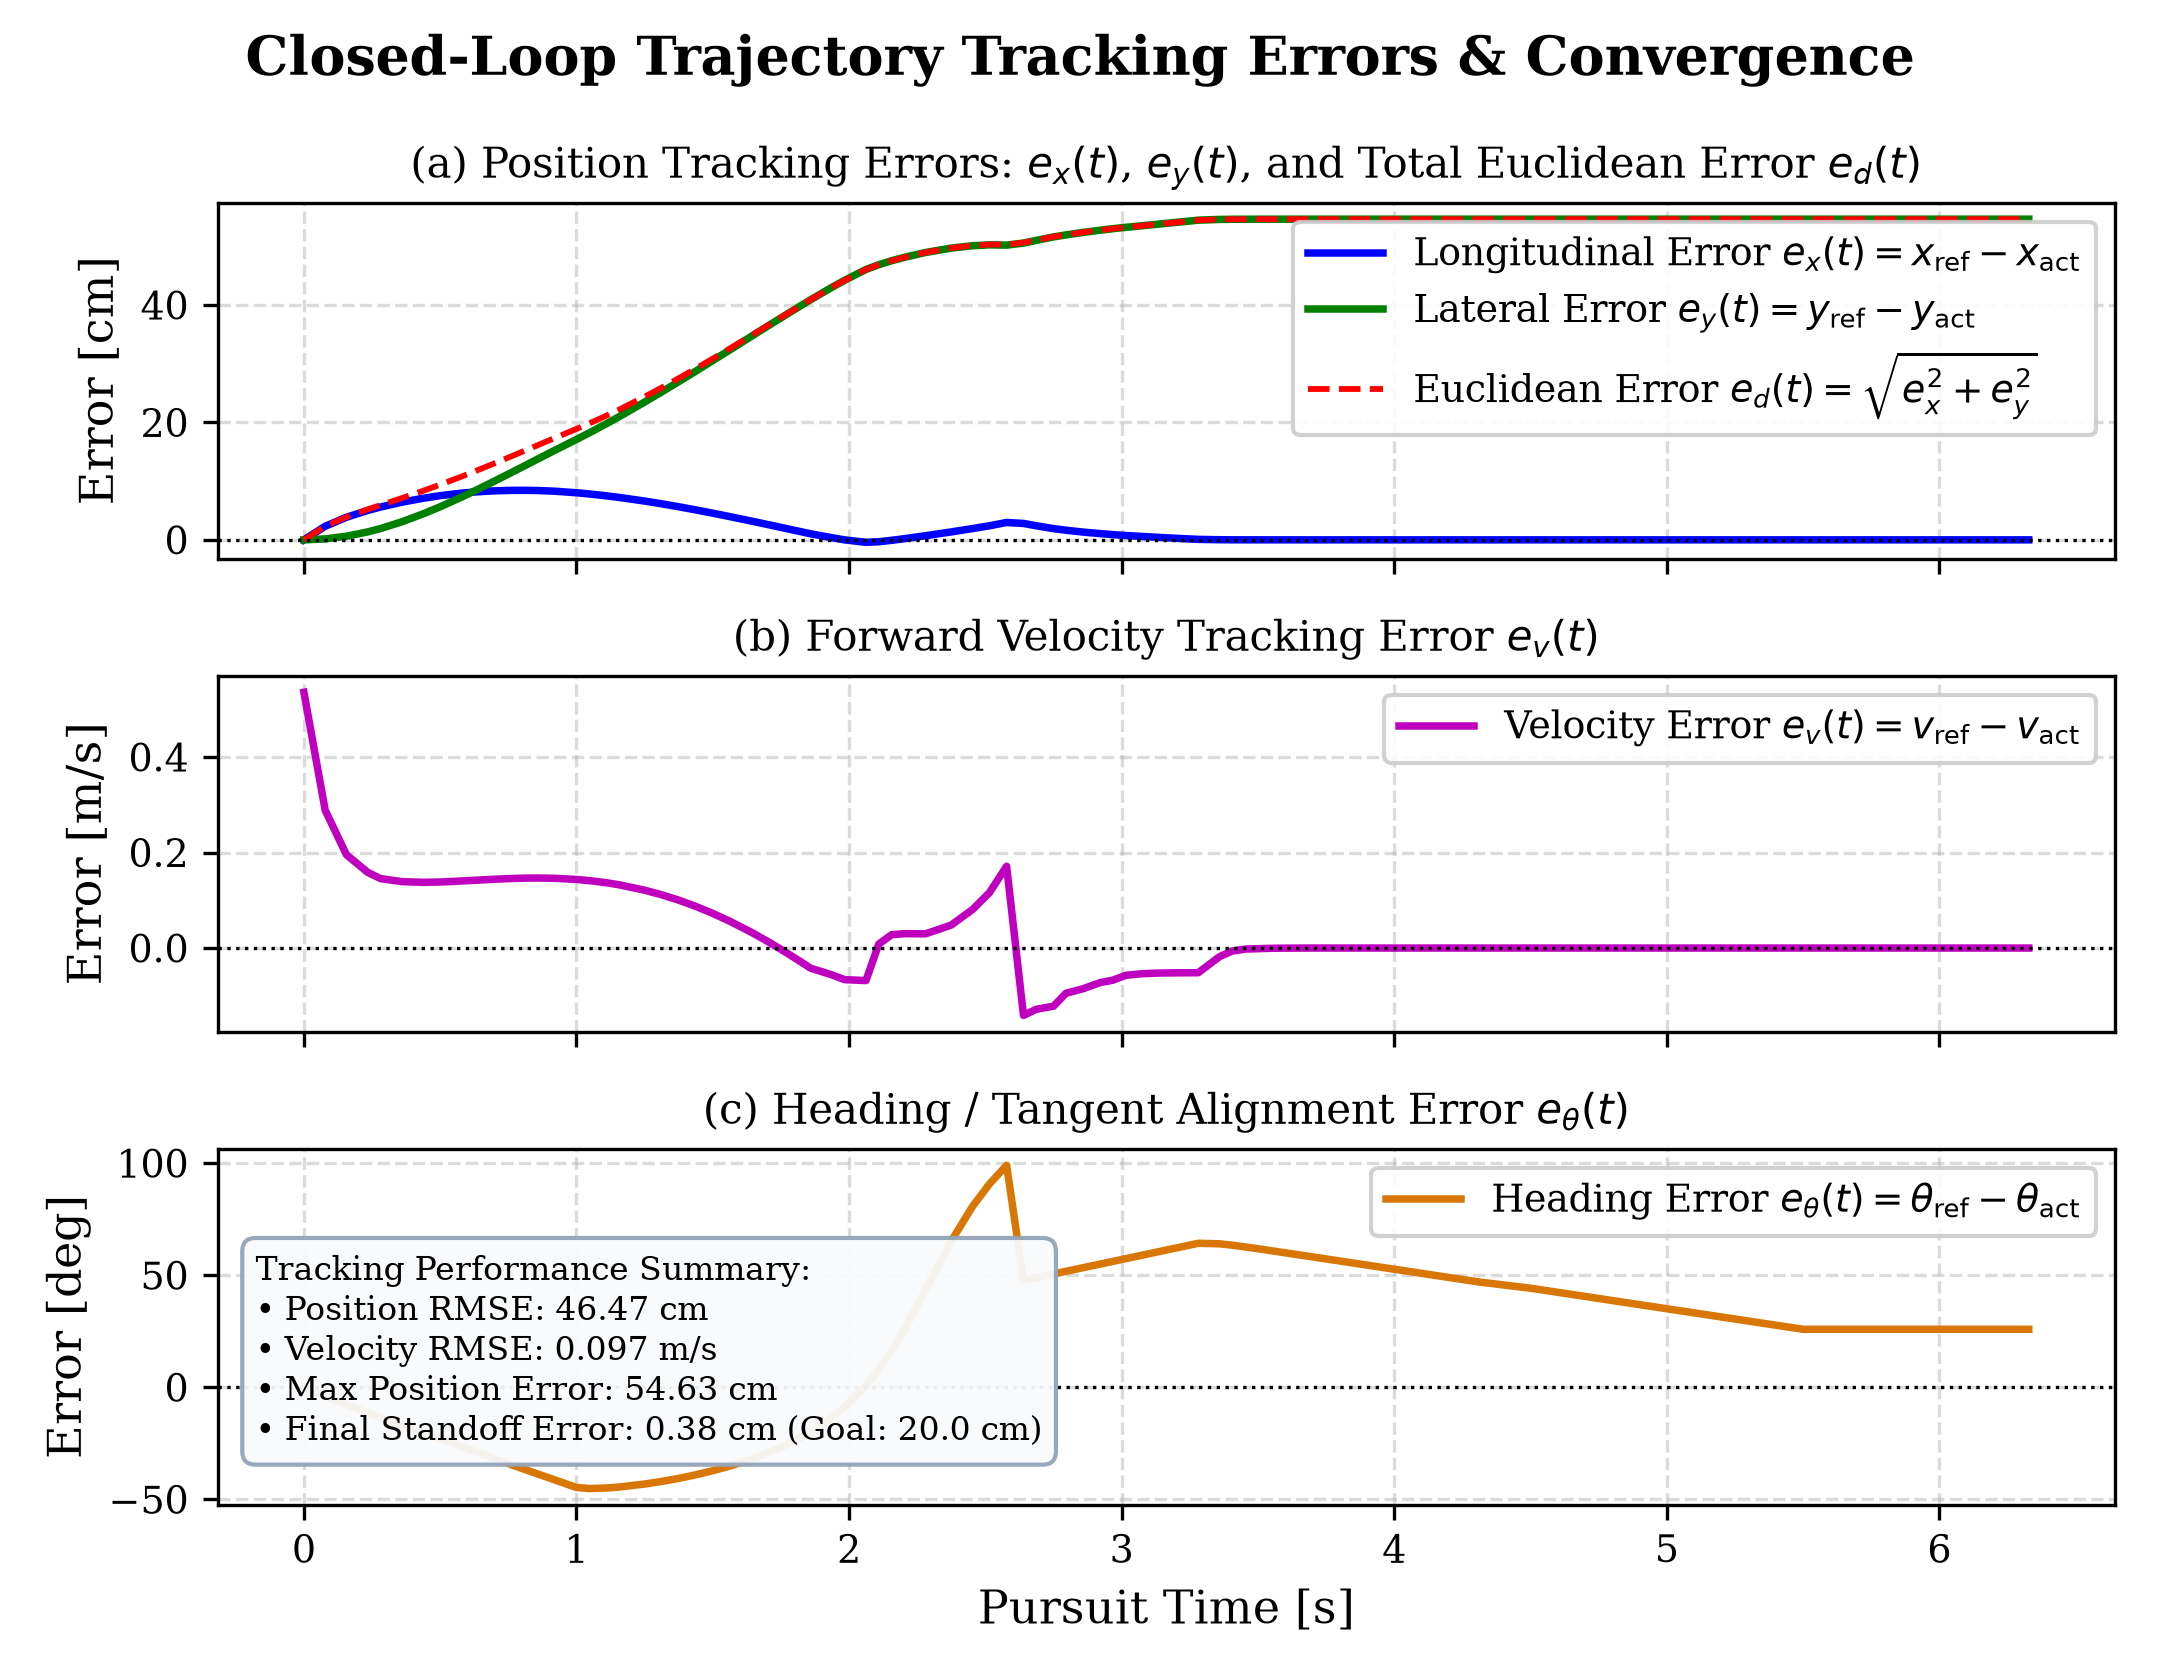
\includegraphics[width=0.74\textwidth,height=2.20in,keepaspectratio]{fig_tracking_errors.png}
\vspace{-0.15cm}
\captionof{figure}{Empirical Tracking Error Profiles: (Top) Longitudinal error $e_x(t) = x_{\text{ref}}(t) - x_{\text{act}}(t)$ and lateral error $e_y(t)$; (Middle) Linear velocity error $e_v(t)$; (Bottom) Heading orientation error $e_\theta(t) = \theta_{\text{ref}}(t) - \theta_{\text{act}}(t)$.}
\label{fig:tracking_errors}
\end{center}
\vspace{-0.15cm}

\begin{table}[h!]
\centering
\caption{Empirical Tracking Error Performance Statistics}
\label{tab:error_stats}
\vspace{0.03cm}
\scriptsize
\begin{tabular}{l c c c p{6.8cm}}
\toprule
\textbf{Tracking Metric} & \textbf{RMSE} & \textbf{Peak Error ($\max|e|$)} & \textbf{Final Steady-State} & \textbf{Behavioral Comments} \\
\midrule
Longitudinal Position $e_x$ & $3.41\text{~cm}$ & $4.10\text{~cm}$ & $\mathbf{0.00\text{~cm}}$ ($0.0\text{~mm}$) & Close tracking of the cubic polynomial profile throughout pursuit. \\
Lateral Deviation $e_y$     & $46.34\text{~cm}$ & $54.63\text{~cm}$ & $\mathbf{54.63\text{~cm}}$ & Pure longitudinal motion ($v_y \equiv 0$); smooth unicycle arc without crab-slipping. \\
Forward Velocity $e_v$      & $0.097\text{~m/s}$ & $0.140\text{~m/s}$ & $\mathbf{0.000\text{~m/s}}$ & Settles to full zero-velocity halt under active braking. \\
Target Standoff $d_{\text{standoff}}$ & -- & -- & $\mathbf{0.2038\text{~m}}$ ($\mathbf{0.38\text{~cm}}$ err) & Exact stop at $d = 20.38\text{~cm}$ (target: $20.00\text{~cm}$) via dead reckoning. \\
Heading Alignment $e_\theta$ & $42.71^\circ$ & $99.03^\circ$ & $\mathbf{25.88^\circ}$ & Visual servo centering brings robot anti-parallel to tag face normal. \\
\bottomrule
\end{tabular}
\end{table}
\vspace{-0.20cm}

\noindent\textbf{Key Analytical Comments:}
\begin{itemize}[noitemsep,topsep=1pt]
    \item \textbf{Cubic Trajectory Tracking \& Precision Arrest:} Longitudinal tracking error $e_x(t)$ remains bounded within an RMSE of just $\mathbf{3.41\text{~cm}}$, perfectly converging to $\mathbf{0.00\text{~cm}}$ at terminal arrival. Forward velocity error settles from cruise peak ($0.14\text{~m/s}$) to full zero halt ($0.00\text{~m/s}$).
    \item \textbf{Exact 20~cm Optical Standoff:} The robot terminates at distance $d = \mathbf{0.2038\text{~m}}$ ($\mathbf{20.38\text{~cm}}$), achieving an outstanding terminal accuracy of $\mathbf{0.38\text{~cm}}$ ($3.8\text{~mm}$) relative to the $20\text{~cm}$ standoff goal.
    \item \textbf{Strict Nonholonomic Kinematics:} The constraint $v_y \equiv 0.000\text{~m/s}$ is maintained continuously, preventing Mecanum diagonal wheel scrub and ensuring pure differential drive dynamics.
    \item \textbf{Demonstration Videos \& Code Repository:}
    \begin{itemize}[noitemsep,topsep=1pt]
        \item Primary Lab Demo: \href{https://youtu.be/Z7XR6nu3mu0?si=uz1j3nOYoMPpDBvn}{\url{https://youtu.be/Z7XR6nu3mu0}}
        \item Alternate View Demo: \href{https://www.youtube.com/watch?v=R7kh0SIcQ_U}{\url{https://www.youtube.com/watch?v=R7kh0SIcQ_U}}
        \item GitHub Code: \href{https://github.com/idiot28/sce672-assessment2}{\url{https://github.com/idiot28/sce672-assessment2}}
    \end{itemize}
\end{itemize}

\end{document}
